
\begin{document}

\maketitle

\section{Sissejuhatus}
\begin{frame}[fragile]
  \frametitle{Täna kavas}
\begin{itemize}
	\item Sissejuhatus (1)
	\begin{itemize}
		\item Tutvumine
		\item Õppe struktuur
		\item Kodukord
		\item Aine struktuur
	\end{itemize}
	\item Äristrateegia ja IT seosed (3)
	\item Arhitektuur (2)
\end{itemize}
	
\end{frame}

\begin{frame}[fragile]
	\frametitle{Andres Kütt}
	\begin{columns}[t]
		\begin{column}{7cm}
			\begin{itemize}
				\item Raha eest programme tegemas alates 1993
				\item Viimased kümmekond aastat arhitekt
				\item $\approx$MSc (UT, Statistika), MBA (EBS), MSc (MIT)
				\item Hetkel Riigi Infosüsteemi arhitekt
				\item Minevikus Skype, Hansapank, EMTA jne. + natuke konsultatsiooni
				\item Palju eri loenguid ja kursusi eri koolides
			\end{itemize}
		\end{column}
		\begin{column}[T]{3cm}
			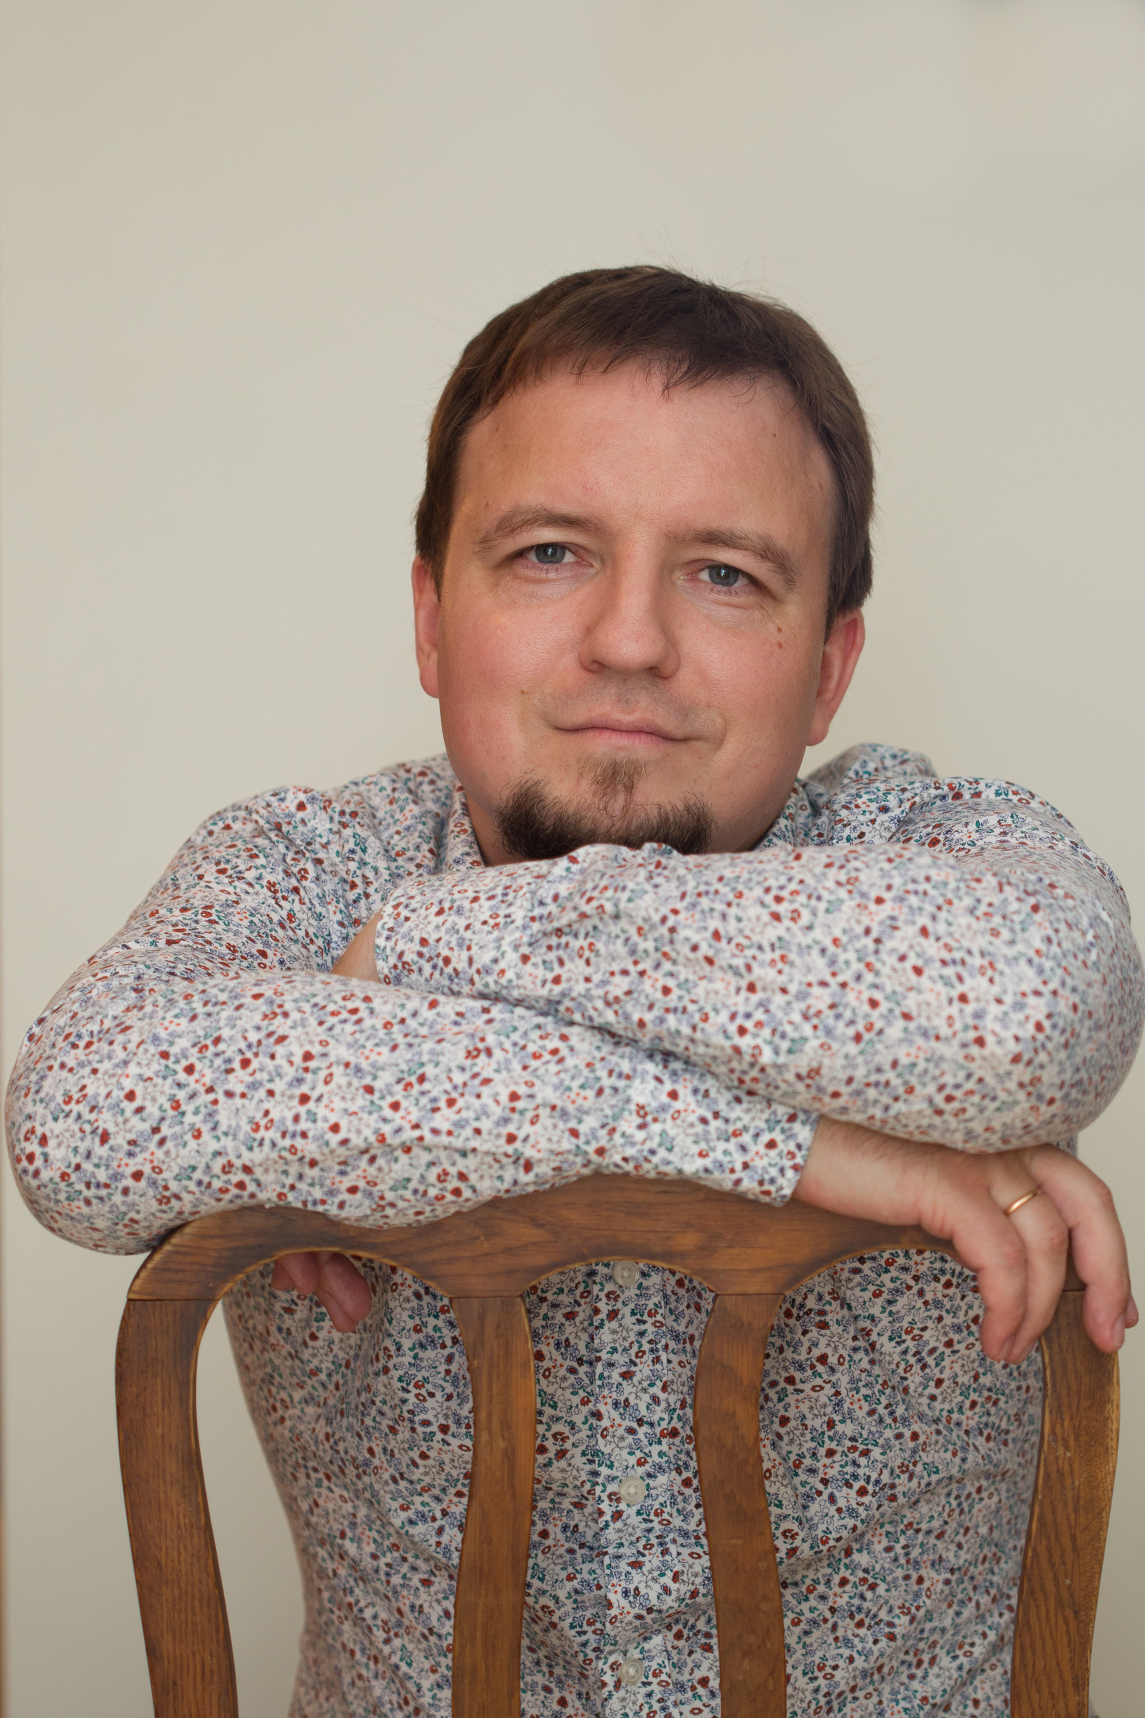
\includegraphics[width=\textwidth]{author.jpg}
		\end{column}
	\end{columns}
\end{frame}

\begin{frame}[fragile]
  \frametitle{Õppe struktuur}
	\begin{itemize}
	\item Loengud
	\begin{itemize}
		\item Igal kohtumisel 6 30-minutilist blokki
		\item Igas blokis 20 minutit juttu, 5 minutit arutelu paarides ja 5 minutit avalikku arutelu
		\item Loengus osalemine ei ole kohustuslik, seminaris osalemine on
	\end{itemize}
	\end{itemize}
\end{frame}

\begin{frame}[fragile]
  \frametitle{Kodutööst}
Eesmärk on läbida IT strateegia koostamine \emph{võimalikult realistlikes} tingimustes 
  	\begin{itemize}
		\item Grupi suurus: $1<N<8$
		\item Äri- ja IT strateegia vahelist piiri ette ei kirjutata
		\item Formaadi osas vabad käed (dokument, esitlus, tants vms.), peab olema vaid taasesitamist võimaldav
		\item Edukriteerium: ettevõttel läheb paremini, kui ilma selle dokumendita
		\item Hindamiskriteerium: ruumis viibijad peavad edu tõenäoliseks
	\end{itemize}
\end{frame}
\note{Kodutöö ja selle ette kandmine on kõige olulisem asi siin aines}

\begin{frame}[fragile]
  \frametitle{Eksamist}
  Eksamiks on kahe või rohkema punktiga kirjalik analüütiline töö
  	\begin{itemize}
		\item Hinnatakse sisu, mitte mahtu
		\item Kogemus võiks toimida: kui vastus on OK, kuid ei tugine loengule kaotab punkte vaid natuke
		\item Kui kodutöö on 100\%, eksamit vaja ei ole
	\end{itemize}
\end{frame}


\begin{frame}[fragile]
  \frametitle{Õppe struktuur. Materjalid}
	\begin{itemize}
		\item Teen slaidid aga juttu läbi ei kirjuta
		\begin{itemize}
			\item Vähemalt ei saa seda lubada
			\item Kui keegi koostab mõistliku konspekti, aitan seda toimetada ja avaldada
			\item Tegelen kursuse raames tehnoloogilise loenguinnovatsiooniga \url{https://github.com/andreskytt/it_strateegia}!
		\end{itemize}
		\item Kõik vabalt saada olevad tekstid tekivad ÕISi
		\item Kohustuslikku kirjandust ei ole sest teema on liiga lai ja inimeste võimalused erinevad
		\item Soovituslikku kirjandust viitan jooksvalt ja panen slaidide lõppu 
		\note{Tekib ka koondbibliograafia\\}
	\end{itemize}
\note{Kogu asi on olemas githubis, sinna võib muutusi teha. Tegu on pedagoogilise eksperimendiga, eks näis, kuidas läheb. }
\end{frame}


\begin{frame}[fragile]
  \frametitle{Kodukord}
	\begin{itemize}
		\item Lubatud
		\begin{itemize}
			\item Küsimused ja õppejõu seisukohtade vaidlustamine
			\item Oma kogemuse mõõdukas jagamine
			\item Saabumine ja lahkumine millal iganes
		\end{itemize}
		\item Keelatud
		\begin{itemize}
			\item Aja raiskamine. Nii teie enese kui meie ühise aja.
		\end{itemize}
	\end{itemize}
\end{frame}
\note{On oluline vahe oma kogemuse jagamisel ja mõõdutul jauramisel, sama käib küsimuste kohta}

\begin{frame}[fragile]
  \frametitle{Aine struktuur}
	\begin{itemize}
		\item Tuginen IT Juhi kutsestandardile \citep{kutsestandard}
			\begin{itemize}
				\item Markeerin teemad, mida mujal kaetakse
				\item Tegelen jõudu mööda katmata teemadega
				\item Annan terviku
			\end{itemize}
		\item Tegelen põhimõtteliste asjadega
			\begin{itemize}
				\item Strateegia ülesandeks on vastata küsimusele “Kuidas me teeme asju paremini, kui teised” \citep{de2006strategy}	
				\item Seega on vaja aru saada aluspõhimõtetest
				\item Pealisehitus on nii ehk naa muutlik ja mitte-akadeemiline
			\end{itemize}
	\end{itemize}
\end{frame}
\note{ITILit, TOGAFi, COBITit, Scrumi jne. jne. jne. saate ise ka uurida. Nende mood muutub ja tegu ei ole akadeemilises mõttes relevantsete asjadega. Teadus on siiski teadus.}

\begin{frame}[fragile]
  \frametitle{Aine struktuur}
		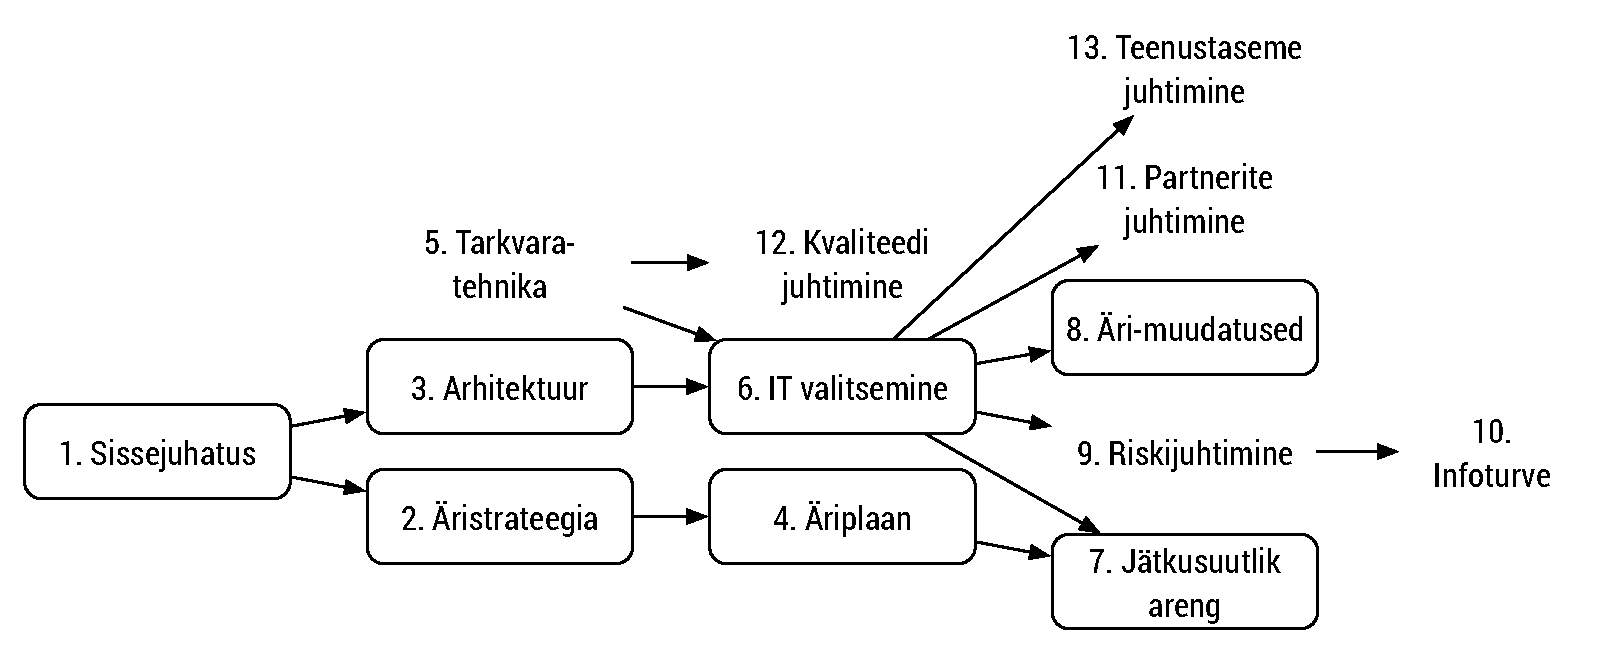
\includegraphics[width=\textwidth]{aine_struktuur.pdf}
\end{frame}
\note{Numbrid näitavad teemade esitamise järjekorda. Kastiga on sügavamalt käsitletavad teemad, ilma on asjad, mida mujal põhjalikult läbi räägitakse}

%Arutelu koht
\begin{frame}[fragile]
  \frametitle{Arutelu koht}
		\begin{center}
			\textbf{Mis on ootused sellele ainele?}
		\end{center}
\end{frame}
		
\section{Äristrateegia ja IT seosed}
\begin{frame}[fragile]
  \frametitle{Mis on strateegia?}
	\begin{itemize}
		\item Definitisioon Kluyver \& Pearce ja selle olulised omadused (erilisus, erinevus taktikast)
	\end{itemize}
\end{frame}

\begin{frame}[fragile]
  \frametitle{Sõjakunst}
  \emph{"Stratagos"} - Kreeka keeles väejuht. Sun Tzu "sõjakunst" \citep{tzu2013art} on siiani rakendatav:
  
  Võidul on viis osist. Võidab see, 
   \begin{enumerate}
   		\item kes teab, millal võidelda ja millal mitte
		\item kes teab, kuidas toimida tugevama ja nõrgema vastasega
		\item kelle armee kõik astmed on täidetud samast vaimust
		\item kes, olles ise valmis, ootab, tabamaks vastane ootamatult
		\item kellel on suveräänist segamata sõjaline võimekus
   \end{enumerate}
\end{frame}

\begin{frame}[fragile]
  \frametitle{Sõjakunst}
  \begin{quote}
    All warfare is based on deception
  \end{quote}

\end{frame}

\begin{frame}[fragile]
  \frametitle{Strateegia laiemas kontekstis}
  Strateegia on osa laiemast organisatsiooni juhtimise süsteemistkuhu kuuluvad veel kindlasti 
  	\begin{description}
		\item[Visioon] kui nägemus ühisest helgest tulevikust
		\item[Missioon] kui põhjus eksisteerida
		\item[Kultuur] kui komplekt kooseksisteerimist võimaldavaid väärtusi
	\end{description}	
	\begin{quote}
	vision = mission + strategy + culture \end{quote}\citep{lipton1996demystifying}
\end{frame}


\begin{frame}[fragile]
  \frametitle{Strateegia dünaamikast}
  Kuna muutub keskkond ja muutub ka organisatsioon, on strateegia olemuselt dünaamiline nähtus. Seega
	\begin{itemize}
		\item Peab strateegiaga kaasas käima selle muutmise või ignoreerimise protsess
		\item Aegub ta varem või hiljem
		\item Tekitab liigne strateegiasse klammerdumine varem või hiljem lõhe juhtkonna ja töötajate vahele
	\end{itemize}
\end{frame}

\begin{frame}[fragile]
  \frametitle{Strateegia olemusest}
  Strateegiaga samaväärselt oluline on tema arendamise protsess. 
	\begin{itemize}
		\item Kasvõi tulenevalt strateegia dünaamilisest olemusest
		\item Ühise suuna määratlemine eeldab, et kuidagi tegeletakse konfliktidega. Vähemalt tulevad need lauale.
		\item Pimedusse on kergem astuda sõbraga õlg õla kõrval. Strateegia arutelu annab kindluse, et ma lähme edasi kõik koos
	\end{itemize}
\end{frame}

\begin{frame}[fragile]
  \frametitle{Strateegia kui jada otsuseid}
	Strateegiat võib vaadelda kui hulka otsuseid. Mida me teeme ja mida me \emph{ei tee}. Järelikult
	\begin{itemize}
		\item on strateegia loomisse, nagu igasse otsusesse, sisse ehitatud konflikt
		\item on strateegia aluseks edasistele otsustele (näiteks: projektide prioriteedid)
		\item ei tohi strateegiadokument olla "ümmargune"
	\end{itemize}
\end{frame}


%Arutelu koht
\begin{frame}[fragile]
  \frametitle{Arutelu koht}
		\begin{center}
			\textbf{Kas üldse saab rääkida IT strateegiast?}
		\end{center}
\end{frame}

\begin{frame}[fragile,label={stack}]
	\frametitle{Organisatsiooni kihiline mudel}
	\begin{columns}[t]
		\begin{column}{6cm}
			\begin{itemize}
				\item Iga kiht on seotud eelmise ja järgmisega
				\item Illustreerib IT asukohta organisatsioonis arhitekti vaatepunktist
				\item Sarnane TOGAFi lähenemisele, kuid laiema tähendusega
			\end{itemize}
		\end{column}
		\begin{column}[T]{5cm}
			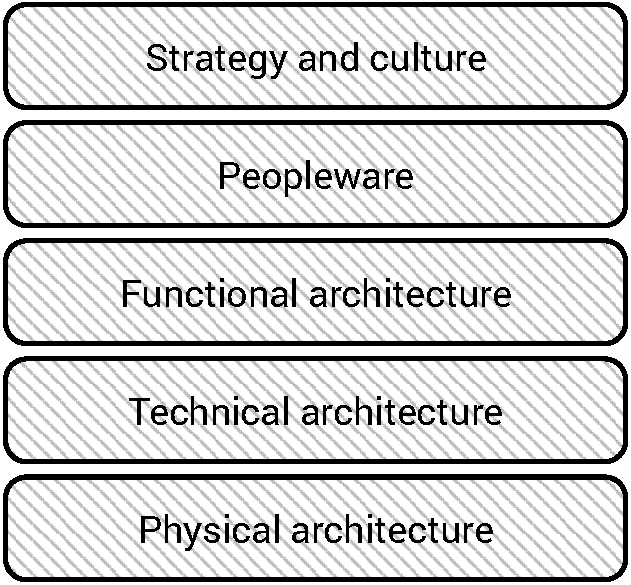
\includegraphics[width=\textwidth]{stack.pdf}
		\end{column}
	\end{columns}
\end{frame}

\begin{frame}[fragile]
  \frametitle{Kihid}
  	\begin{description}
		\item[Äri ja juriidika] Organisatsiooni strateegia ja juriidiline kontekst (seadusandlus, lepingud jne.)
		\item[Organisatsioon ja protsessid] Strateegiat realiseerivad org. struktuur ja äriprotsessid. Ka kultuur.
		\item[Funktsionaalsed komponendid] Protsesse toetavad funktsionaalsed komponendid (näiteks e-mail, ERP, veebipood, tootmisliin)
		\item[Tehnilised lahendused/IT] Funktsinaalsete komponentide tehniline/tehnoloogiline realisatsioon
		\item[Taristu] Tehniliste lahenduste taristu kuid ka näiteks kontorihooned
	\end{description}
\end{frame}

\begin{frame}[fragile]
  \frametitle{Järeldused mudelist}
	\begin{itemize}
		\item Kõik kihid on \emph{pidevas} muutumises, organisatsioon on dünaamiline nähtus
		\item Ükski muutus ei leia aset vaid ühes kihis
		\item Isoleeritud muutused tekitavad "tektoonilisi pingeid"
		\item Muutused propageeruvad üles ja alla tavaliselt kahaneva mõjuga
		\item IT ja äri kihid tavaliselt \emph{ainsad} üheselt juhitavad
	\end{itemize}
\end{frame}

%Arutelu koht
\begin{frame}[fragile]
  \frametitle{Arutelu koht}
		\begin{center}
			\textbf{Kui kiiresti muutused sumbuvad? Kas äristrateegia muutus võib muuta majutus-strateegiat?}
		\end{center}
\end{frame}

\begin{frame}[fragile]
  \frametitle{IT ja äri joondamine}
  IT eri aspektid ja organisatsioon toimivad pidevas dünaamilises tasakaalus. Vt. \cite{luftman2004assessing}
	\begin{columns}[t]
		\begin{column}{6cm}
			\begin{itemize}
				\item Osapooltel on vastandlikud huvid
				\item Oluline on huvide tasakaal
				\item Tasakaal tekib läbi organisatsiooni struktuuri ja protsesside
			\end{itemize}
		\end{column}
		\begin{column}[T]{5cm}
			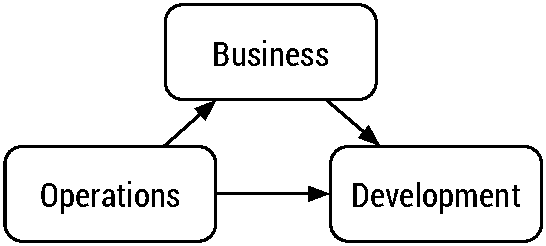
\includegraphics[width=\textwidth]{alignment.pdf}
		\end{column}
	\end{columns}
\end{frame}

\begin{frame}[fragile]
  \frametitle{IT kui integraalne osa organisatsioonist}
  Infotehnoloogiata ei ole mõeldavad terve rida organisatsiooni protsesse, ITl on nende kaudu oluline mõju äri toimivusele.
	\begin{itemize}
		\item ERP\footnote{Enterprise Resource Planning}
		\item Info/teadmus juhtimine
		\item Äriprotsesside juhtimine
	\end{itemize}
\end{frame}

\begin{frame}[fragile]
  \frametitle{IT mõju läbi {ERPi}}
  ERPi abil käivad ettevõtte paljud võtmeprotsessid: finants- ja personalijuhtimine, laohaldus jne. 
	\begin{itemize}
		\item ERPi suhteliselt väike probleem omab laialdast mõju
		\item Ettevõtte paindlikkus sõltub tema võimest muutusi ERPis kajastada
	\end{itemize}
  IT mõju näited:
	\begin{itemize}
		\item Milline partner või partnerid valitakse tarkvara pakkuma? 
		\item Kas ehitatame ise või ostame?
		\item Kuidas lahendatakse kasutajatoe ja majutuse küsimused? 
	\end{itemize}

\end{frame}

\begin{frame}[fragile]
  \frametitle{IT mõju läbi teadmusjuhtimise}
  Teadmus on ettevõtte jaoks kriitiline konkurentsieelis \citep{david2000diagnosing}. Tema juhtimine ilma tehnoloogiata ei ole lahenduv ülesanne. 
  	\begin{itemize}
		\item Loe teadmusjuhtimisest ja selle tehnilistest aspektidest \citep{15.905}
		\item Peamine järeldus: me ei saa teadmusjuhtimisest aru ja tegemist on kriitilise funktsiooniga. Seega tuleb talle läheneda väga ettevaatlikult.
	\end{itemize}
\end{frame}

\begin{frame}[fragile]
  \frametitle{IT mõju läbi äriprotsesside juhtimise}
		\begin{center}
			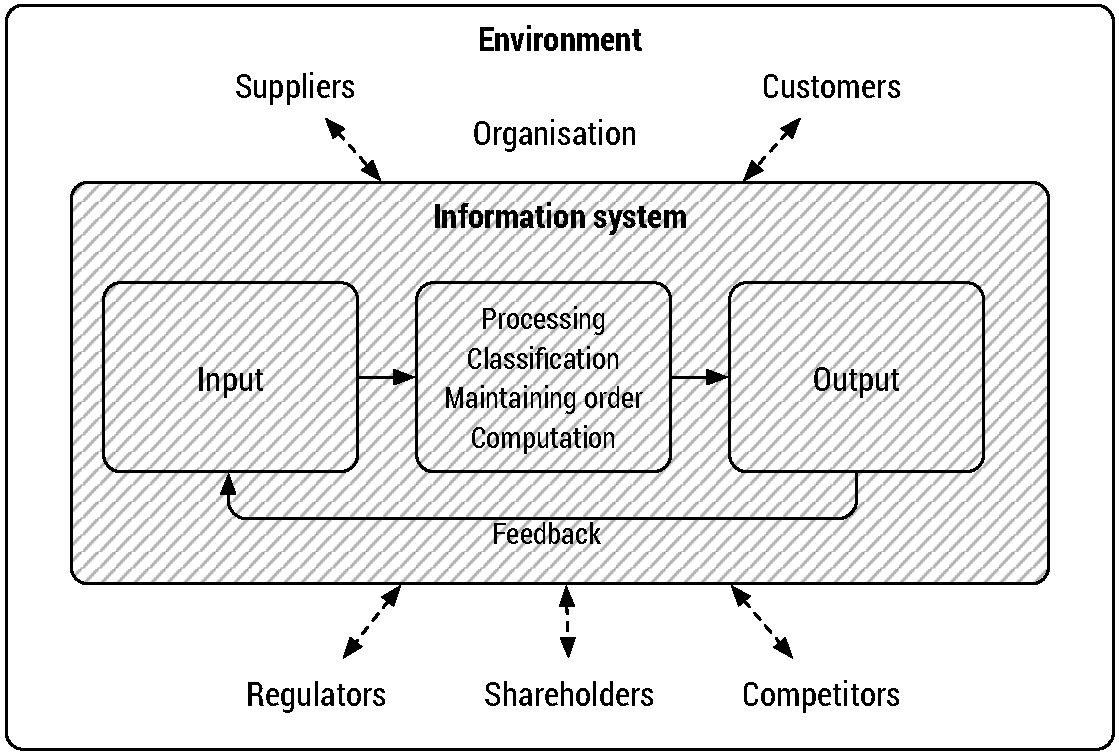
\includegraphics[width=.80\textwidth]{info_org.pdf}\\
		\end{center}
		\cite{laudon2000management}
\end{frame}


%Arutelu koht
\begin{frame}[fragile]
  \frametitle{Arutelu koht}
		\begin{center}
			\textbf{Kas saab olla mõistlikku IT juhtimist kui organisatsioon kui tervik ei ole mõistlikult juhitud?}
		\end{center}
\end{frame}

\section{Arhitektuur}

\begin{frame}[fragile]
  \frametitle{Arhitektuuri tavapärane käsitlus}
		Inseneri vaates on arhitektuur kirjeldus sellest, kuidas millegi osad omavahel sobivad
		\begin{itemize}
			\item Toimiv ja end tõestanud praktika
			\item Hea arusaam tapi tugevusest ei anna vastust küsimusele, kuidas ehitada hea maja
		\end{itemize}
		
		Akadeemilises vaates on arhitektuur tavaliselt viis millegi formaalseks kirjeldamiseks ja selle kirjelduseni jõudmiseks
		\begin{itemize}
			\item Väga palju tööd millest väga vähe jõuab praktikasse
			\item Terve hulk omavahel sobimatuid paradigmasid
			\item Aitab mõelda vaid formaliseeritavatest asjadest
		\end{itemize}
		
\end{frame}

\begin{frame}[fragile]
	\frametitle{Vitruvius Pollio}
	\begin{columns}[t]
		\begin{column}{7cm}
			\begin{center}
				\begin{quote}
					\ldots all these must be built with due reference to durability, convenience and beauty
				\end{quote}
			\end{center}
			\vskip 1cm
			Marcus Vitruvius Pollio, 80-70 eKr.- 15 pKr  \citep{pollio1914vitruvius}
		\end{column}
		\begin{column}[T]{3cm}
			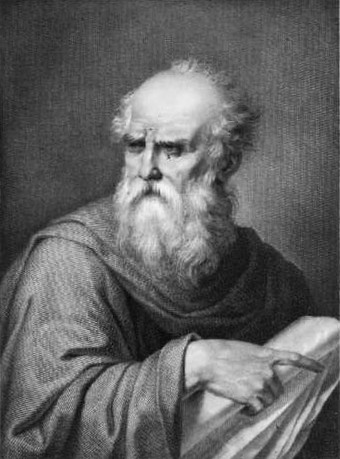
\includegraphics[width=\textwidth]{vitruvio.jpg}
		\end{column}
	\end{columns}
\end{frame}

\begin{frame}[fragile]
  \frametitle{Süsteemi definitsioon}
		\begin{center}
  			\begin{quote}
				Süsteem on selgelt piiritletud hulk omavahelises vastasmõjus olevaid elemente.
			\end{quote}
		\end{center}
\end{frame}

\begin{frame}[fragile]
  \frametitle{Süsteemi piiridest}
		Igasugune süsteemi piiri tõmbamine on meelevaldne
		\begin{itemize}
			\item Tavaliselt tõmmatakse piir kas kontrolli või tehnoloogia alusel, vt. ka slaid \ref{Yosemite}
			\item Süsteemi võib kuuluda nii riistvara, tarkvara kui inimesed ning nedevahelised suhted
			\item Järelikult ei saa rääkida vaid tarkvara või näiteks laua arhitektuurist, vt. ka slaid \ref{stack}
		\end{itemize}

\end{frame}

\begin{frame}[fragile]
  \frametitle{Arhitekti palve}
		\begin{center}
  			\begin{quote}
				Anna mulle jõudu muuta asju, mida ma muuta saan, kannatlikkust mitte muuta asju, mida ma muuta ei saa ning eelkõige anna mulle tarkust nende kahe vahel vahet teha
			\end{quote}
		\end{center}
\end{frame}

\begin{frame}[label=Yosemite]
	\frametitle{Yosemite näide süsteemi piiridest}
	\begin{columns}[t]
		\begin{column}{6.5cm}
			Apple muutis 2013. teises pooles põhjalikult OS Xi kiipkaardi draiveriarhitektuuri
			\begin{itemize}
				\item Baastarkvaras muutust teha ei jõutud 
				\item 1. detsembril esimesed e-residendid
				\item Tulemuseks kallis ja närvesööv rabelemine
			\end{itemize}
		\end{column}
		\begin{column}[T]{4.5cm}
			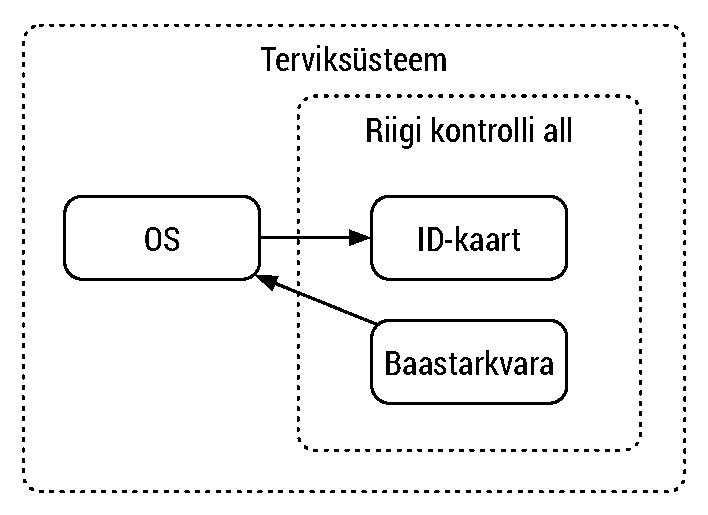
\includegraphics[width=\textwidth]{yosemite.pdf}
		\end{column}
	\end{columns}
\end{frame}

%Arutelu koht
\begin{frame}[fragile]
  \frametitle{Arutelu koht}
		\begin{center}
			\textbf{Millist väärtust loob arhitektuuriga tegelemine?}
		\end{center}
\end{frame}

\begin{frame}
	\frametitle{Alternatiivne arhitektuuri käsitlus}
	Ed Crawley pakub käsitlust, mis eelkirjeldatute probleemid ületab
	\begin{columns}[t]
		\begin{column}{6cm}
			\begin{itemize}
				\item Tervikuks seotakse nii süsteemi funktsionaalsed kui tehnilised aspektid 
				\item Mudel arvestab konteksti
				\item Praktikas kasutusel, akadeemias siiski vähem
				\item Paraku korralikult avaldamata
			\end{itemize}
		\end{column}
		\begin{column}[T]{4cm}
			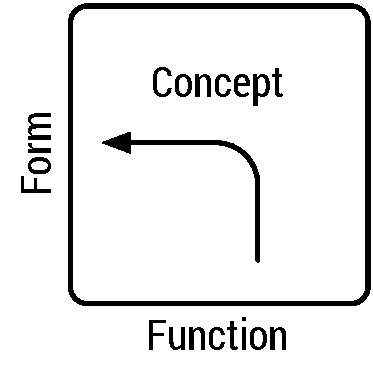
\includegraphics[width=\textwidth]{ffc.pdf}
		\end{column}
	\end{columns}

\end{frame}


\begin{frame}[fragile]
  \frametitle{Architecture is...}
  		\begin{center}
			\begin{quote}
			The embodiment of \textbf{concept}, and the allocation of physical/informational \textbf{function} to elements of \textbf{form}, and definition of \textbf{interfaces} among the elements and with the surrounding \textbf{context}.
			\end{quote}
		\end{center}
	\cite{edcrawley} 
\end{frame}

\begin{frame}[fragile]
  \frametitle{Definitsioonid}
	\begin{description}
		\item[Vorm] See, mis \emph{on} + selle miski struktuur
		\item[Funktsioon] See, mida tehakse struktureerituna peamist väärtust toova protsessi ümber
		\item[Kontseptsioon] Süsteemi visioon, mis seob vormi funktsiooniga ning kehastab peamisi printsiipe
	\end{description}
\end{frame}
\note{Kontseptsioon on see koht, kus mängu tuleb organisatsiooni kultuur, selle asjaga me veel kohtume! Just see vastab küsimusele, miks mõistlik lahendus samala probleemile on startupis ja pangas erinev}

\begin{frame}[fragile]
  \frametitle{Märkused mudeli kohta}
	\begin{itemize}
		\item Arhitektuur määrab disaini- ja operatiivparameetrid, disain annab neile väärtused
		\item Kuna mudel sisaldab nii funktsiooni kui vormi struktuuri, on mudel tihedalt seotud keerukuse kontseptsiooniga
		\item Väga multidistiplinaarne lähenemine (inseneriteadus, juhtimine, kontrolliteooria, AI, matemaatika jne.)
		\item Olemuslikult holistiline ja seotud süsteemimõtlemisega 
	\end{itemize}
\end{frame}

%Arutelu koht
\begin{frame}[fragile]
  \frametitle{Arutelu koht}
		\begin{center}
			\textbf{Kui palju erineb toodud mudel harjumuspärasest?}
		\end{center}
\end{frame}

\section{Viited}

\begin{frame}[t,allowframebreaks,]
  	\bibliographystyle{plainnat}
	\bibliography{it_strateegia} 

\end{frame}

\section{Litsents}
\begin{frame}{Theme}

  Get the source of this theme and the demo presentation from

  \begin{center}\url{github.com/matze/mtheme}\end{center}

  The theme \emph{itself} is licensed under a
  \href{http://creativecommons.org/licenses/by-sa/4.0/}{Creative Commons
  Attribution-ShareAlike 4.0 International License}.

  \begin{center}\ccbysa\end{center}

\end{frame}

\begin{frame}{Sisu}
	The contents of the slides is lidecensed under a \href{http://creativecommons.org/licenses/by-nc-sa/4.0/}{Creative Commons Attribution-NonCommercial-ShareAlike 4.0 International}
	\begin{center}\ccbyncsa\end{center}
\end{frame}

%\plain{Küsimusi?}
\begin{frame}[plain]
	\begin{center}Küsimusi?\end{center}
\end{frame}


\begin{frame}[fragile]
  \frametitle{Lahtised otsad ja ideed}
	\begin{itemize}
		\item Arthur Ganson Machine with Concrete kui näide muutuste põhjustest
		\item Keerukus ärimuutuste juures rääkida
		\item Iga loengu algusse slaid asukohaga skeemil
		\item \url{http://www.wired.com/2014/12/disappearing-business-of-design} näide ärimuutustest. Tehnilise kihi piirilt üles ja alla tagasi
		\item Nordea näide ärimuudatustega reageerimise juurde (oluline on kiirendus, mitte niivõrd kiirus)
	\end{itemize}
\end{frame}


\end{document}